
% this file is called up by thesis.tex
% content in this file will be fed into the main document

%: ----------------------- introduction file header -----------------------
\chapter{Introduction}
\label{chapterIntroduction}
% the code below specifies where the figures are stored
\ifpdf
    \graphicspath{{Intro/fig/PNG/}{Intro/figDF/}{Intro/fig/}}
\else
    \graphicspath{{Intro/fig/EPS/}{Intro/fig/}}
\fi

% ----------------------------------------------------------------------
%: ----------------------- introduction content ----------------------- 
% ----------------------------------------------------------------------



%: ----------------------- HELP: latex document organisation
% the commands below help you to subdivide and organise your thesis
%    \chapter{}       = level 1, top level
%    \section{}       = level 2
%    \subsection{}    = level 3
%    \subsubsection{} = level 4
% note that everything after the percentage sign is hidden from output


% ----------------------------------------------------------------------
\section{Background} 
% ----------------------------------------------------------------------

% ----------------------------------------------------------------------
\section{Approaches} 
% ----------------------------------------------------------------------
%%%%%%%%%%%%%%%%%%%%%%%%%%%%%%%%%%%%%%%%%%%%
%\begin{figure}[htbp]
%\setbox0\vbox{
%\centering{\scalebox{0.5}[0.5]{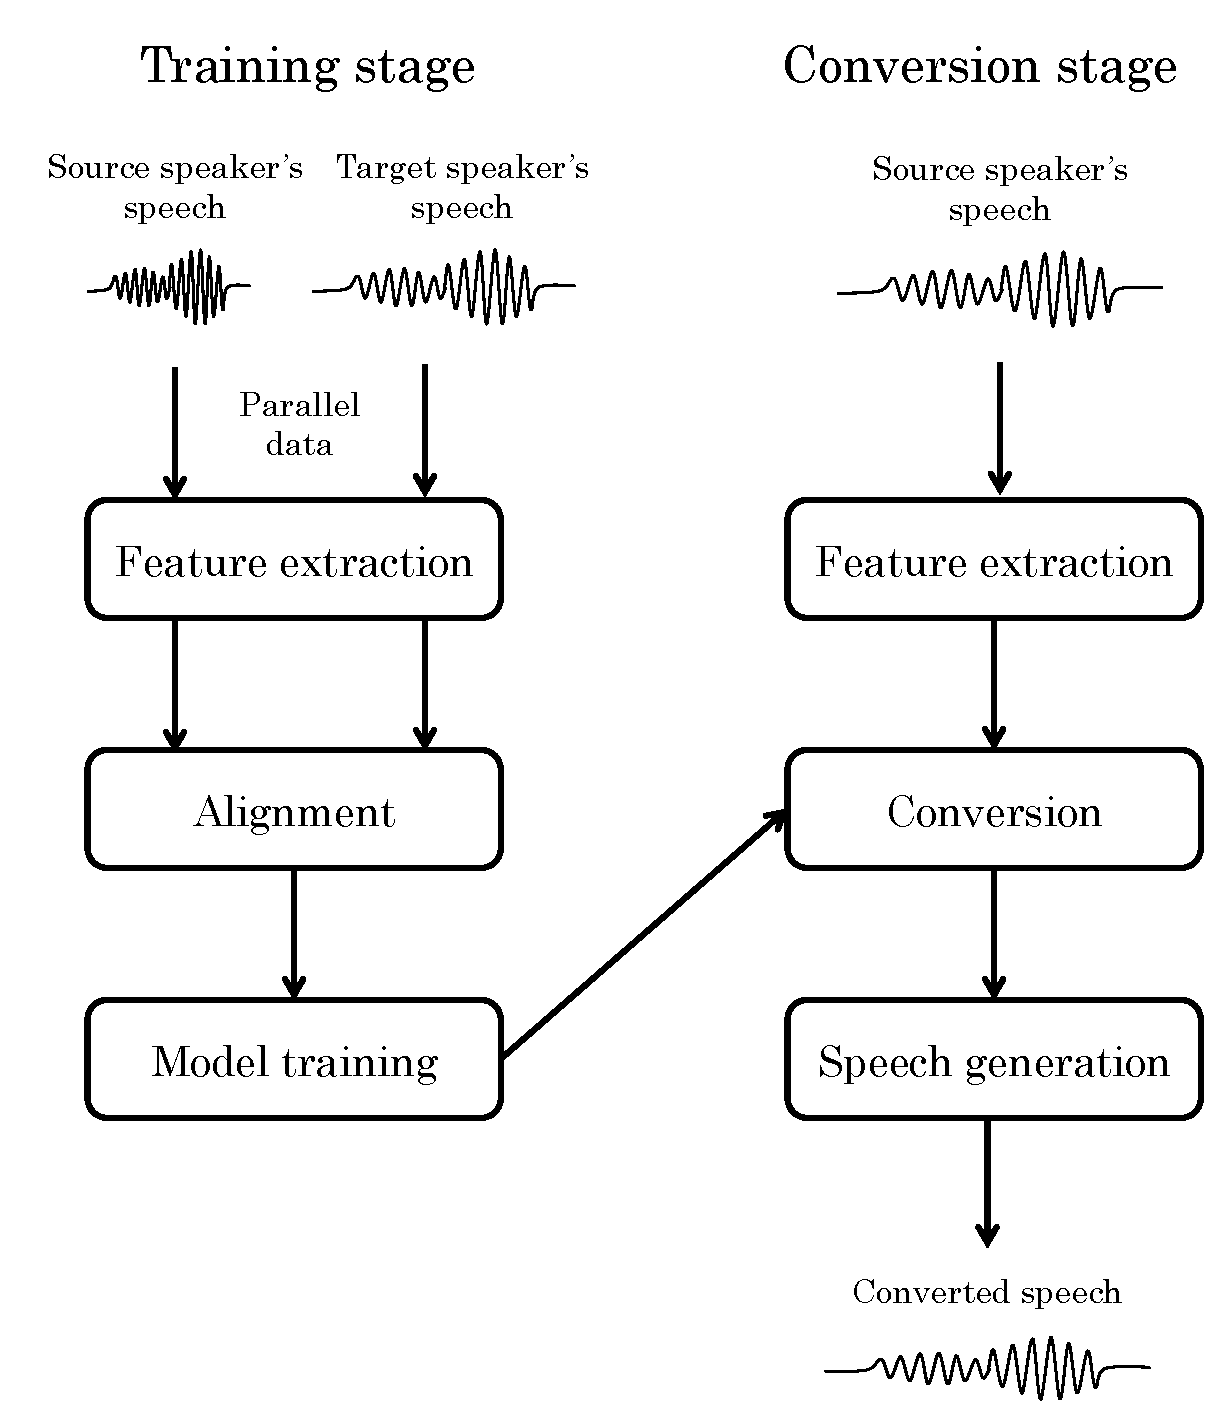
\includegraphics{vc_flow.eps}}}
%}
%\centerline{\box0}
%\caption{Flowchart of a typical VC system}
%\label{fig:vc_flow}
%\end{figure}
%%%%%%%%%%%%%%%%%%%%%%%%%%%%%%%%%%%%%%%%%%%%

% ----------------------------------------------------------------------
\section{Purpose of This Thesis} 
% ----------------------------------------------------------------------

% : --------------------------------------------
\subsection{Four Practical VC Tasks} 
% : --------------------------------------------
% # -----------------------------------------
\subsubsection{Noise-robust VC} 
% # -----------------------------------------

% # -----------------------------------------
\subsubsection{Assistive Technology for Articulation Disorders} 
% # -----------------------------------------

% # -----------------------------------------
\subsubsection{VC Using Small-parallel Training Data} 
% # -----------------------------------------

% # -----------------------------------------
\subsubsection{Many-to-many VC} 
% # -----------------------------------------

% : --------------------------------------------
\subsection{Novelties of This Thesis} 
% : --------------------------------------------

% ----------------------------------------------------------------------
\section{Outline} 
% ----------------------------------------------------------------------

